\normallinespacing

\chapter{The Reinforcement Learning Paradigm}

Reinforcement Learning (RL) is a sub-field of machine learning wherein an agent learns to take optimal decision in an unknown environment by trial and error.
RL differs from the other branches of machine learning -- namely supervised learning and unsupervised learning.
Supervised learning involves learning from labeled data whereas unsupervised learning involves finding the underlying structure of unlabeled data.
RL involves an agent actively exploring an interactive environment sequentially and
performing actions to maximize a "reward" metric over a number of steps.

\begin{figure}[!htbp]
    \centering
    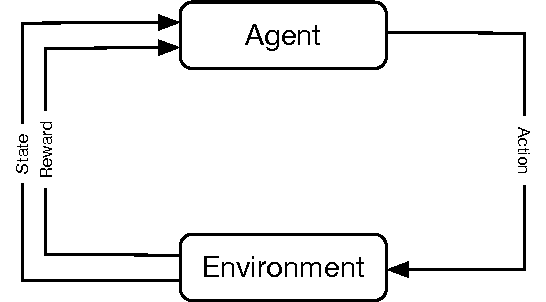
\includegraphics{rl/rl_scheme.pdf}
    \caption{The basic reinforcement learning scheme.}
    \label{fig:rl_scheme}
\end{figure}

In the RL paradigm, at each time step, an agent interacts with the environment by choosing an action based on its present state using a learned policy $\pi$.
Then the agent transitions onto a new state as dictated by the dynamics of the environment.
It receives a scalar feedback, a reward, pertaining to its previous action in the process.
This chapter serves as a brief introduction to the reinforcement learning paradigm and introduces its various components that will be used throughout the manuscript.

\section{Markov Decision Processes}

A typical model of an environment in RL task is represented as a Markov Decision Processes (MDP).
To achieve a goal in a MDP, the learning agent has to learn the parameter of the MDP and take optimal decisions based on these learned parameters.
Formally, an MDP, $M$, in the discounted reward setting, is defined as the quintuple $M = \langle \mathcal{S}, \mathcal{A}, \mathcal{R}, \mathcal{P} \rangle$, where the various components are defined as follows:

\subsection{Set of States}

A state is a representation of the agent's environment.
The state of states that the MDP can be in is denoted by $\mathcal{S}$.

\subsection{Set of Actions}

It is a set of possible moves available to the agent at any state, denoted by the set $\mathcal{A}$.
Taking an action may cause the agent to transition from one state to another.

\subsection{Reward}

It is a scalar feedback received from the environment as a consequence of the agent's action.
A characteristic of reinforcement learning is the delayed rewards.
It means that the consequence of an action is not immediate, its effect is observed in the future.

\subsection{Transition Probabilities}

$\mathcal{P}$ is a transition probability kernel.
$\mathcal{P}(s^\prime \mid s, a)$ denotes the probability of transitioning from state $s$ to another state $s^\prime$ after an action $a$ is executed.

\section{Action Policy}

Policy $\pi$ characterizes the behavior of the learning agent in a state $s$. 
It qualifies the action(s) that the agent will undertake in a particular state $s$.

A policy can be \textbf{stochastic}, it induces a probability distribution over the set of actions $\mathcal{A}$ for a given state s.

A policy may be \textbf{deterministic}, it maps each state from the set of states $\mathcal{S}$ to a single action from the set of actions $\mathcal{A}$.

A policy may \textbf{depend} on the sequence of all previous states, i.e. the \textbf{history}, that the learner has visited. 

A policy may also be \textbf{Markov} (where that current state is a sufficient statistic of the previous states), it only depends on the current state $s$ that the learner is in.

A policy is \textbf{stationary} if it does not change over time.

\section{Objective}

The objective in the RL problem is to maximize a intrinsic reward metric subject to the dynamics of the environment governed by its underlying MDP.

The objective for the average reward setting is formally defined as
Starting from state $s$ following the policy $\pi$, formally the average reward objective to maximize is defined as
$$\lim_{T \to \infty} \mathbb{E}\left[\frac{1}{T} \sum_{t=1}^{T} R_t \mid S_0 = s\right]$$
where, $T$ is the time horizon.

Other settings such as discounted reward, cumulative reward settings also exist in reinforcement learning but we will be focusing in the average reward setting in this work.

\section{Gain}

The gain ($\rho$) or the expected value function of an MDP starting at state $s$ in the infinite-horizon setting with average rewards is formally defined as
$$\rho(s) = \max_\pi \mathbb{E}\left[\lim_{T \to \infty} \frac{1}{T} \sum_{t=1}^{T} R_t \mid S_0 = s\right]$$

\section{Value Function}

The value of a state $s$ under a policy $\pi$, $V_\pi(s)$, is defined as the reward that can be accumulated starting from that state and taking actions according to the policy $\pi$. 

\section{Optimality}

\subsection{Optimal Policy}

A policy $\pi$ is better than another policy $\pi^\prime$ if and only if for all states, following policy $\pi$ yields a value such that $V_\pi(s) \ge V_{\pi^\prime} (s)$.
A policy $\pi^*$ is optimal if is better than all other policies.

\subsection{Optimal Value Function}

The value function induced by following the optimal policy is the optimal value function. Formally it is defined as
$$V^*(s) = \max_\pi V_\pi(s)$$

\section{MDP Classes}

MDPs can be classified into various categories based on its transition probability and the policy being executed. They are briefly described below.

\subsection{Communicating States}

Two states $s_1$ and $s_2$ in an MDP are said to be communicating under a policy $\pi$ if there is a non-zero probability of reaching each state from the other in zero or more state transitions.

\subsection{Recurrent States}

A state $s$ is recurrent if there is a non-zero probability of returning to the same state under a policy $\pi$ in zero or more state transitions.
In other words, the probability of eventually returning to state $s$ is unity.

\subsection{Ergodic Class of States}

A subset of states are said to belong to an ergodic class if they are recurrent, communicate with each other and do not communicate with any states outside the class.
A Markov chain is irreducible if $\mathcal{S}$, the set of all states, forms an ergodic class.

\subsection{Ergodic MDP}

An MDP is ergodic if the transition matrix corresponding to every policy has a single recurrent class of states.

\subsection{Communicating MDP}

An MDP is communicating if each pair of states communicate with each other under some stationary policy $\pi$.

\section{Bellman Equations and Optimality}

\subsection{Bellman Equations for Evaluating a Policy}

The gain of a policy $\pi$ is defined as 
$$\rho^\pi(s) = \mathbb{E}^\pi\left[\lim_{T \to \infty} \frac{1}{T} \sum_{t=1}^{T} R_t \mid S_0 = s\right]$$.

The bias of a policy $\pi$ is the measure of the total deviation of the reward from the asymptotic average reward.
It is formally defines as
$$h^\pi(s) = \mathbb{E}^\pi\left[\lim_{T \to \infty} \sum_{t=1}^{T} (R_t - \rho^\pi(S_t) \mid S_0 = s\right]$$

Assuming a policy $\pi$ such that all states are reachable from a single recurrent class, then the Bellman equation is defined as

\begin{equation}
    \label{eqn:bellman_eq}
    h^\pi(s) - \rho^\pi(s) = \mathbb{E}_{a \sim \pi(\cdot \mid s), s^\prime \sim \mathcal{P}(\cdot \mid  s, a)} \left[ R(s, a, s^\prime) + h^\pi(s^\prime) \right]
\end{equation}

Equation \ref{eqn:bellman_eq} can be compactly written as $h^\pi - \rho^\pi = R^\pi + \mathcal{P}^\pi h^\pi$ and is the Bellman equation for evaluating a policy $\pi$.

\subsection{Bellman Optimality Equations}

Assuming communicating MDPs, Puterman \cite{puterman_chapter_1990} showed that for the optimal gain policy, the optimal average infinite horizon reward does not depend on the starting state. In other words, $\rho^*(s) = \rho^*$.

For a communicating MDP, let $h^*$ be the bias of the optimal policy $\pi^* = \arg \max_\pi \rho^\pi$ and $\rho^*$ be the optimal gain. 
Then, the Bellman optimality equations state that the optimal gain $\rho^* = \rho$ is a feasible solution of the equations below 

\begin{equation}
    \rho + h(s) = \max_a R(s, a) + \sum_{s^\prime} P(s, a, s^\prime) h^*(s) \quad \forall s \in \mathcal{S}
\end{equation}

\section{Value Iteration}

From the recursive definition of the Bellman optimality equation, an iterative algorithm can be formulated. 
This is motivated by the fact that using dynamic programming approaches is infeasible for computationally large state, action spaces and large or infinite time horizons.
One such algorithm is the value iteration algorithm. The value iteration algorithm for the average reward scenario as proposed by Hordijk and Tijms \cite{hordijk_modified_1975} is described as follows

\subsubsection*{Pseudocode}
\begin{enumerate}
    \item Start with a vector of values $\mathbf{v}_0$
    \item Repeat until convergence 
    
    \begin{itemize}
        \item For each state $s \in \mathcal{S}$
        $$\mathbf{v}_t(s) = \max_a \left(r(s, a) + \alpha_t \sum_{s^\prime} \mathcal{P}(s^\prime \mid s, a) \mathbf{v}_{t-1}(s^\prime) \right)$$
        where $\alpha_t \to 1$ as $t \to \infty$
    \end{itemize}
    
    
    \item Finally, the optimal policy is computed as
    $$\pi(s) \in \arg_a\max r(s,a) + \mathbf{P}(s,a)^\top \mathbf{v}_k(s) $$
    
\end{enumerate}

Value iteration converges to an optimal policy in a finite number of iterations if there exists a state $s$ that is reachable from all other states under all stationary policies.
Value iteration cannot discriminate between gain optimal and bias optimal policies.

% Links - 
% https://ieor8100.github.io/rl/docs/Lecture%201%20-MDP.pdf
% http://proceedings.mlr.press/v119/bourel20a/bourel20a.pdf
% https://arxiv.org/pdf/2009.04575.pdf

